%% Standalone lecture -- build with:  pdflatex -shell-escape kernelTrick
%% Shared preamble for standalone lecture files.
%%
%% Every lecture begins with %% Shared preamble for standalone lecture files.
%%
%% Every lecture begins with %% Shared preamble for standalone lecture files.
%%
%% Every lecture begins with \input{preamble} and is compiled on its own:
%%     pdflatex -shell-escape <lecture>
%% There is no master lectures.tex any more -- the list of lectures lives in
%% lectures.yaml and is read by the build scripts.

\documentclass[25pt,landscape,footrule]{foils}
\input{macros_gen}
\backgroundsetup{contents={}}

\usepackage{stmaryrd}
\usepackage{ifthen}
\usepackage{pdf14}

% Every figure lives in this course's lectures/figures (consolidated
% 2026-10-08).  Do not add other courses' folders back: when a name exists in
% several folders LaTeX silently takes the first, which mixed old and new
% frames of the same animation.  A missing figure should be a build error.
\graphicspath{{figures/}{../lectures/figures/}}

\date{}

\newcounter{lessoncnt}
\newcommand{\lesson}[1]{\setcounter{page}{1}%
\section{Mathematics of Machine Learning\\%
\vfill
\textcolor{red}{\textit{#1}}
\vfill}}
 and is compiled on its own:
%%     pdflatex -shell-escape <lecture>
%% There is no master lectures.tex any more -- the list of lectures lives in
%% lectures.yaml and is read by the build scripts.

\documentclass[25pt,landscape,footrule]{foils}
%\usepackage[compat2,pdftex]{geometry}
\usepackage[pdftex]{geometry}
\geometry{headsep=-2.5ex,hscale=0.9,bmargin=2.5cm,tmargin=1cm,textwidth=25cm}
\usepackage[pdftex]{xcolor}
\usepackage{pause}
\usepackage{background}
%\usepackage[color=white]{background}
\usepackage{listings}
\usepackage{graphicx}
\usepackage{epsfig}
\usepackage{epstopdf}
\usepackage{bm}
\usepackage{amssymb}
\usepackage{amsfonts}
\usepackage{marvosym}
\usepackage{cite}
\usepackage{pifont}
\usepackage[english]{babel}
\usepackage{amsmath}
\usepackage{amsfonts}
\usepackage{rotating}
\usepackage{listings}
\usepackage{pp4slide}
%\usepackage{hyperref}
\usepackage{pp4link}
\usepackage{fancyvrb}
\usepackage{multido}
\usepackage{calc}
\usepackage{mleftright}
\mleftright % Redefines \left to \mleft and \right to \mright



\thinmuskip=1mu

\newcommand{\bigstrut}{\rule[-0.5\baselineskip]{0pt}{1.2\baselineskip}}
\renewcommand{\ttdefault}{pcr}

\newcommand{\squeeze}{\setlength{\itemsep}{-2pt}}
%\renewcommand{\familydefault}{cmr}
%\renewcommand{\labelitemii}{\textcolor{green}{$\star$}}
\newcommand{\tick}{{\large \ding{51}}}
\newcommand{\cross}{{\large \ding{55}}}
%\DeclareMathAlphabet{\mat}{OT1}{cmss}{bx}{n}
\DeclareMathAlphabet{\mat}{U}{eur}{b}{n}
\newcommand{\figs}{/home/apb/figures}
\newcommand{\stimes}{{\scriptstyle \times}}
\newcommand{\tr}{\textsf{T}}
\newcommand{\e}[1]{{\rm e}^{#1}}
\newcommand{\E}[1]{{\rm e}^{{\displaystyle #1}}}
\newcommand{\av}[2][]{\mathbb{E}_{#1}\left[ #2 \right]}
\newcommand{\Var}[1]{\mathbb{V}\mathrm{ar}\left( #1 \right)}
\newcommand{\pred}[1]{\left\llbracket { \small #1} \right\rrbracket}
\newcommand{\logg}[1]{\log\left( #1 \right)}
\newcommand{\logtwo}[1]{\log_2\left( #1 \right)}
\newcommand{\bra}[1]{\left( #1 \right)}
\newcommand{\prob}[1]{\mathbb{P}\left( #1 \right)}
\newcommand{\Prob}[1]{\mathbb{P}\left( #1 \right)}
\newcommand{\Step}{\mathop{\mat{\Theta}}}
\newcommand\diag{\mathop{\mathrm{diag}}}
\newcommand{\grad}{\bm{\nabla}}
\newcommand{\gradx}{\bm{\nabla}_{\!\!\scriptscriptstyle \bm{x}}}
\newcommand{\gradw}{\bm{\nabla}_{\!\!\scriptscriptstyle \bm{w}}}
\newcommand{\dd}{\mathrm{d}}
\newcommand{\ii}{\mathrm{i}}
\newcommand{\data}{\mathcal{D}}
\newcommand{\class}{\mathcal{C}}
\newcommand{\hypo}{\mathcal{H}}
\newcommand{\indep}{\perp \!\!\!\! \perp}
\newcommand{\pd}[3][\,]{\frac{\partial^{#1}{#2}}{\partial\,{#3}}}
\newcommand{\normal}[1]{\mathcal{N}\!\left( #1 \right)}
\newcommand{\Dist}[2][Binom]{\mathrm{#1}\left( \strut {#2} \right)}
\newcommand{\brackets}[1]{\!\left( #1 \right)}
\newcommand{\KL}[2]{\mathop{\mathrm{KL}}\left(#1 \big\| #2\right)}
\newcommand{\argmax}{\mathop{\mathrm{argmax}}}
\newcommand{\argmin}{\mathop{\mathrm{argmin}}}
\newcommand{\margin}{\Delta}
\lstnewenvironment{matlab}[1][frame=TB]{\lstset{#1}}{}       
%\renewcommand{\emph}[1]{\textcolor{red}{\textbf{#1}}}
\newcommand{\myskip}[1]{}
\newcommand\mycom[2]{\genfrac{}{}{0pt}{}{#1}{#2}}
\newcommand{\jl}{\lstinline[basicstyle=\ttfamily\color{DarkGreen},%
 keywordstyle=\bfseries\ttfamily\color{DarkGreen}]}
\definecolor{EmphColor}{rgb}{0.0,0.0,1.0}
\renewcommand{\emph}[1]{{\color{EmphColor}\textbf{#1}}}
\newcommand{\len}[1]{\| #1 \|}
\newcommand{\inner}[2]{\left\langle {#1}, {#2}\right\rangle}
\newenvironment{psmallmatrix}{\left(\begin{smallmatrix}}{\end{smallmatrix}\right)}
  

\definecolor{DarkGreen}{rgb}{0,0.5,0}
\definecolor{DarkRed}{rgb}{0,0,0.5}
\definecolor{HighLight}{rgb}{1,0,0}     % yellow
\definecolor{TextColor}{rgb}{0.0,0.1,0.1}     % white
\definecolor{TwoColor}{rgb}{0.0,0.5,0.1}      % used for switching colors

\definecolor{HeadLineColor}{rgb}{1.0,0.0,0.0} % cyan
\definecolor{SpecialColor}{rgb}{0.53,0.81,1.0}
\renewcommand{\normalcolor}{\color{HeadLineColor}}

\pausecolors{TwoColor}{TextColor}{HighLight}
\pausecolors{EmphColor}{TextColor}{EmphColor}
\pausecolors{DarkGreen}{DarkGreen}{DarkRed}
\pausecolors{SpecialColor}{white}{HighLight}

\newenvironment{PauseHighLight}{\color{TwoColor}\pausehighlight}{}
\newcommand{\multipdf}[2][width=\linewidth]{\multiinclude[pause=\pauselevel{:+0}\pause,format=pdf,graphics={#1}]{#2}}

\lstdefinelanguage{pseudo}
 {keywords={all,and,begin,break,continue,do,else,elseif,%
     end,endif,endfor,endwhile,%
     exit,false,for,forall,goto,if,%
     or,return,then,true,to,repeat,until,while},%
  comment=[s]{/*}{*/},%
  morecomment=[l]//,%
  morestring=[d]"%
 }[keywords,comments,strings]


\lstloadlanguages{Java,pseudo,Python}
\lstset{
  basicstyle=\footnotesize\ttfamily\color{DarkGreen},
  keywordstyle=\bfseries\footnotesize\ttfamily\color{DarkGreen},
  commentstyle=\footnotesize\it\rmfamily\color{blue},
  language=Java,
  showstringspaces=false
  }


\lstnewenvironment{pseudo}[1][]{\lstset{language=pseudo,mathescape,literate={:=}{{$\gets$}}2 {!}{{$\neg$}}1 {!=}{{\!\!$\neq$\,\,}}2 {<=}{{\!\!$\leq$\,\,}}2 {>=}{{\!\!$\geq$\,\,}}2,escapechar=\#,#1}}{}
\lstnewenvironment{java}[1][]{\lstset{escapechar=\$,#1}}{}
% Python code: the language setting makes # comments use commentstyle.
% Comments stay monospaced: the default italic roman letter-spaces badly
% on listings' fixed columns.
\lstnewenvironment{python}[1][frame=TB]{\lstset{language=Python,
    commentstyle=\footnotesize\ttfamily\color{blue},#1}}{}

\MyLogo{}
%\Restriction{}
%\rightfooter{\hyperlink{overview}{$\square$}}

\newcommand{\keywords}[1]{\vfill{\noindent\it #1}}

\newcounter{outlineitem}
\setcounter{outlineitem}{0}
\newcommand{\outlineitem}[2]{\item%
  \def\targ{\value{emumi}}%
  \ifnum\value{enumi}=\value{outlineitem}%
  \color{HighLight}\textbf{#1}\toptarget{#2}\color{TextColor}%
   \else\toplink{#2}{#1}\fi
}
\color{TwoColor}


%-- Instead of writing \section we want the file structured by \section.
\newcommand{\section}[2][0]{\foilhead[#1cm]{#2}}

%-- Write each page into a \begin{slide} -- \end{slide} environment.
\newenvironment{slide}{}{\pauselevel{=1}}

\MyLogo{\pauselevel{=1}\Acrobatmenu{GoBack}{%
  \color{TextColor}{Adam Pr\"ugel-Bennett}} \hspace{2cm}
  % Clicking on the name steps one slide back.
  \toplink{firstoutline}{\color{red}Mathematics of Machine
    Learning}%
  \hspace{2cm}
  \texttt{//ecs-vlc.github.io/aice3001/}
  %Clicking on the date jumps to the last page, which should be the
  %table of contents.
  \rightfooter{\Acrobatmenu{LastPage}{\qquad%
  \textsf{\color{TextColor}\tiny\thepage}}}% page number
  % Clicking on the page number steps one slide back.
}
\raggedright
\newcommand{\Outline}{}

\newcommand{\pb}{\pausebuild \color{TwoColor}}
\newcommand{\pauseb}{\pauselevel{build, highlight}\pause}
\newcommand{\hl}[1]{\pauselevel{=1, highlight =1 :1, highlight =#1 :#1}\pause}
\newcommand{\hll}{\pauselevel{=1, highlight =1 :1}\pause}
\newcommand{\pauseh}{\pauselevel{highlight}\pause}
\newcommand{\nhl}[1]{\textcolor{TextColor}{#1}}
\newcommand{\mypl}[1]{\pauselevel{=#1 :#1}\pause}
\input supp-pdf.tex
\DeclareGraphicsRule{*}{mps}{*}{}
\usepackage{mpmulti}
%\leftheader{}
\rightheader{} % no more page numbers on top right


\hypersetup{pdftitle={ECS Lectures},pdfsubject={Machine Learning}
pdfauthor={Adam Prugel-Bennett},pdfkeywords={machine learning},
pdfpagemode={FullScreen},
bookmarksopen=false,
hypertexnames=false,pdfstartview={FitV},colorlinks,linkcolor={blue},
citecolor={green},urlcolor={blue}}



\newcommand\bluepage{
\clearpage
\renewcommand\normalcolor{\color{yellow}}
\pagecolor{blue}
\renewcommand\Black{\color{white}}
\color{white}
\hypersetup{colorlinks=true}
}

\newcommand\whitepage{
\clearpage
\renewcommand\normalcolor{\color{black}}
\pagecolor{white}
\renewcommand\Black{\color{black}}
\color{black}
\hypersetup{colorlinks=true}
}

\whitepage
\setlength{\unitlength}{1mm}

\newenvironment{leftImage}[2][0.3]{%
\begin{minipage}{#1\linewidth}
  \includegraphics[width=\linewidth]{#2}
\end{minipage}\hfill
\begin{minipage}{0.92\linewidth - #1\linewidth}}%
{\end{minipage}}

\newenvironment{rightImage}[2][0.3]{%
\newcommand{\foot}{\begin{minipage}{#1\linewidth}\includegraphics[width=0.98\linewidth]{#2}\end{minipage}}%
\begin{minipage}{0.95\linewidth - #1\linewidth}\raggedright }{\end{minipage}\hfill\foot}


%%% Local Variables: 
%%% mode: latex
%%% TeX-master: t
%%% End: 

\backgroundsetup{contents={}}

\usepackage{stmaryrd}
\usepackage{ifthen}
\usepackage{pdf14}

% Every figure lives in this course's lectures/figures (consolidated
% 2026-10-08).  Do not add other courses' folders back: when a name exists in
% several folders LaTeX silently takes the first, which mixed old and new
% frames of the same animation.  A missing figure should be a build error.
\graphicspath{{figures/}{../lectures/figures/}}

\date{}

\newcounter{lessoncnt}
\newcommand{\lesson}[1]{\setcounter{page}{1}%
\section{Mathematics of Machine Learning\\%
\vfill
\textcolor{red}{\textit{#1}}
\vfill}}
 and is compiled on its own:
%%     pdflatex -shell-escape <lecture>
%% There is no master lectures.tex any more -- the list of lectures lives in
%% lectures.yaml and is read by the build scripts.

\documentclass[25pt,landscape,footrule]{foils}
%\usepackage[compat2,pdftex]{geometry}
\usepackage[pdftex]{geometry}
\geometry{headsep=-2.5ex,hscale=0.9,bmargin=2.5cm,tmargin=1cm,textwidth=25cm}
\usepackage[pdftex]{xcolor}
\usepackage{pause}
\usepackage{background}
%\usepackage[color=white]{background}
\usepackage{listings}
\usepackage{graphicx}
\usepackage{epsfig}
\usepackage{epstopdf}
\usepackage{bm}
\usepackage{amssymb}
\usepackage{amsfonts}
\usepackage{marvosym}
\usepackage{cite}
\usepackage{pifont}
\usepackage[english]{babel}
\usepackage{amsmath}
\usepackage{amsfonts}
\usepackage{rotating}
\usepackage{listings}
\usepackage{pp4slide}
%\usepackage{hyperref}
\usepackage{pp4link}
\usepackage{fancyvrb}
\usepackage{multido}
\usepackage{calc}
\usepackage{mleftright}
\mleftright % Redefines \left to \mleft and \right to \mright



\thinmuskip=1mu

\newcommand{\bigstrut}{\rule[-0.5\baselineskip]{0pt}{1.2\baselineskip}}
\renewcommand{\ttdefault}{pcr}

\newcommand{\squeeze}{\setlength{\itemsep}{-2pt}}
%\renewcommand{\familydefault}{cmr}
%\renewcommand{\labelitemii}{\textcolor{green}{$\star$}}
\newcommand{\tick}{{\large \ding{51}}}
\newcommand{\cross}{{\large \ding{55}}}
%\DeclareMathAlphabet{\mat}{OT1}{cmss}{bx}{n}
\DeclareMathAlphabet{\mat}{U}{eur}{b}{n}
\newcommand{\figs}{/home/apb/figures}
\newcommand{\stimes}{{\scriptstyle \times}}
\newcommand{\tr}{\textsf{T}}
\newcommand{\e}[1]{{\rm e}^{#1}}
\newcommand{\E}[1]{{\rm e}^{{\displaystyle #1}}}
\newcommand{\av}[2][]{\mathbb{E}_{#1}\left[ #2 \right]}
\newcommand{\Var}[1]{\mathbb{V}\mathrm{ar}\left( #1 \right)}
\newcommand{\pred}[1]{\left\llbracket { \small #1} \right\rrbracket}
\newcommand{\logg}[1]{\log\left( #1 \right)}
\newcommand{\logtwo}[1]{\log_2\left( #1 \right)}
\newcommand{\bra}[1]{\left( #1 \right)}
\newcommand{\prob}[1]{\mathbb{P}\left( #1 \right)}
\newcommand{\Prob}[1]{\mathbb{P}\left( #1 \right)}
\newcommand{\Step}{\mathop{\mat{\Theta}}}
\newcommand\diag{\mathop{\mathrm{diag}}}
\newcommand{\grad}{\bm{\nabla}}
\newcommand{\gradx}{\bm{\nabla}_{\!\!\scriptscriptstyle \bm{x}}}
\newcommand{\gradw}{\bm{\nabla}_{\!\!\scriptscriptstyle \bm{w}}}
\newcommand{\dd}{\mathrm{d}}
\newcommand{\ii}{\mathrm{i}}
\newcommand{\data}{\mathcal{D}}
\newcommand{\class}{\mathcal{C}}
\newcommand{\hypo}{\mathcal{H}}
\newcommand{\indep}{\perp \!\!\!\! \perp}
\newcommand{\pd}[3][\,]{\frac{\partial^{#1}{#2}}{\partial\,{#3}}}
\newcommand{\normal}[1]{\mathcal{N}\!\left( #1 \right)}
\newcommand{\Dist}[2][Binom]{\mathrm{#1}\left( \strut {#2} \right)}
\newcommand{\brackets}[1]{\!\left( #1 \right)}
\newcommand{\KL}[2]{\mathop{\mathrm{KL}}\left(#1 \big\| #2\right)}
\newcommand{\argmax}{\mathop{\mathrm{argmax}}}
\newcommand{\argmin}{\mathop{\mathrm{argmin}}}
\newcommand{\margin}{\Delta}
\lstnewenvironment{matlab}[1][frame=TB]{\lstset{#1}}{}       
%\renewcommand{\emph}[1]{\textcolor{red}{\textbf{#1}}}
\newcommand{\myskip}[1]{}
\newcommand\mycom[2]{\genfrac{}{}{0pt}{}{#1}{#2}}
\newcommand{\jl}{\lstinline[basicstyle=\ttfamily\color{DarkGreen},%
 keywordstyle=\bfseries\ttfamily\color{DarkGreen}]}
\definecolor{EmphColor}{rgb}{0.0,0.0,1.0}
\renewcommand{\emph}[1]{{\color{EmphColor}\textbf{#1}}}
\newcommand{\len}[1]{\| #1 \|}
\newcommand{\inner}[2]{\left\langle {#1}, {#2}\right\rangle}
\newenvironment{psmallmatrix}{\left(\begin{smallmatrix}}{\end{smallmatrix}\right)}
  

\definecolor{DarkGreen}{rgb}{0,0.5,0}
\definecolor{DarkRed}{rgb}{0,0,0.5}
\definecolor{HighLight}{rgb}{1,0,0}     % yellow
\definecolor{TextColor}{rgb}{0.0,0.1,0.1}     % white
\definecolor{TwoColor}{rgb}{0.0,0.5,0.1}      % used for switching colors

\definecolor{HeadLineColor}{rgb}{1.0,0.0,0.0} % cyan
\definecolor{SpecialColor}{rgb}{0.53,0.81,1.0}
\renewcommand{\normalcolor}{\color{HeadLineColor}}

\pausecolors{TwoColor}{TextColor}{HighLight}
\pausecolors{EmphColor}{TextColor}{EmphColor}
\pausecolors{DarkGreen}{DarkGreen}{DarkRed}
\pausecolors{SpecialColor}{white}{HighLight}

\newenvironment{PauseHighLight}{\color{TwoColor}\pausehighlight}{}
\newcommand{\multipdf}[2][width=\linewidth]{\multiinclude[pause=\pauselevel{:+0}\pause,format=pdf,graphics={#1}]{#2}}

\lstdefinelanguage{pseudo}
 {keywords={all,and,begin,break,continue,do,else,elseif,%
     end,endif,endfor,endwhile,%
     exit,false,for,forall,goto,if,%
     or,return,then,true,to,repeat,until,while},%
  comment=[s]{/*}{*/},%
  morecomment=[l]//,%
  morestring=[d]"%
 }[keywords,comments,strings]


\lstloadlanguages{Java,pseudo,Python}
\lstset{
  basicstyle=\footnotesize\ttfamily\color{DarkGreen},
  keywordstyle=\bfseries\footnotesize\ttfamily\color{DarkGreen},
  commentstyle=\footnotesize\it\rmfamily\color{blue},
  language=Java,
  showstringspaces=false
  }


\lstnewenvironment{pseudo}[1][]{\lstset{language=pseudo,mathescape,literate={:=}{{$\gets$}}2 {!}{{$\neg$}}1 {!=}{{\!\!$\neq$\,\,}}2 {<=}{{\!\!$\leq$\,\,}}2 {>=}{{\!\!$\geq$\,\,}}2,escapechar=\#,#1}}{}
\lstnewenvironment{java}[1][]{\lstset{escapechar=\$,#1}}{}
% Python code: the language setting makes # comments use commentstyle.
% Comments stay monospaced: the default italic roman letter-spaces badly
% on listings' fixed columns.
\lstnewenvironment{python}[1][frame=TB]{\lstset{language=Python,
    commentstyle=\footnotesize\ttfamily\color{blue},#1}}{}

\MyLogo{}
%\Restriction{}
%\rightfooter{\hyperlink{overview}{$\square$}}

\newcommand{\keywords}[1]{\vfill{\noindent\it #1}}

\newcounter{outlineitem}
\setcounter{outlineitem}{0}
\newcommand{\outlineitem}[2]{\item%
  \def\targ{\value{emumi}}%
  \ifnum\value{enumi}=\value{outlineitem}%
  \color{HighLight}\textbf{#1}\toptarget{#2}\color{TextColor}%
   \else\toplink{#2}{#1}\fi
}
\color{TwoColor}


%-- Instead of writing \section we want the file structured by \section.
\newcommand{\section}[2][0]{\foilhead[#1cm]{#2}}

%-- Write each page into a \begin{slide} -- \end{slide} environment.
\newenvironment{slide}{}{\pauselevel{=1}}

\MyLogo{\pauselevel{=1}\Acrobatmenu{GoBack}{%
  \color{TextColor}{Adam Pr\"ugel-Bennett}} \hspace{2cm}
  % Clicking on the name steps one slide back.
  \toplink{firstoutline}{\color{red}Mathematics of Machine
    Learning}%
  \hspace{2cm}
  \texttt{//ecs-vlc.github.io/aice3001/}
  %Clicking on the date jumps to the last page, which should be the
  %table of contents.
  \rightfooter{\Acrobatmenu{LastPage}{\qquad%
  \textsf{\color{TextColor}\tiny\thepage}}}% page number
  % Clicking on the page number steps one slide back.
}
\raggedright
\newcommand{\Outline}{}

\newcommand{\pb}{\pausebuild \color{TwoColor}}
\newcommand{\pauseb}{\pauselevel{build, highlight}\pause}
\newcommand{\hl}[1]{\pauselevel{=1, highlight =1 :1, highlight =#1 :#1}\pause}
\newcommand{\hll}{\pauselevel{=1, highlight =1 :1}\pause}
\newcommand{\pauseh}{\pauselevel{highlight}\pause}
\newcommand{\nhl}[1]{\textcolor{TextColor}{#1}}
\newcommand{\mypl}[1]{\pauselevel{=#1 :#1}\pause}
\input supp-pdf.tex
\DeclareGraphicsRule{*}{mps}{*}{}
\usepackage{mpmulti}
%\leftheader{}
\rightheader{} % no more page numbers on top right


\hypersetup{pdftitle={ECS Lectures},pdfsubject={Machine Learning}
pdfauthor={Adam Prugel-Bennett},pdfkeywords={machine learning},
pdfpagemode={FullScreen},
bookmarksopen=false,
hypertexnames=false,pdfstartview={FitV},colorlinks,linkcolor={blue},
citecolor={green},urlcolor={blue}}



\newcommand\bluepage{
\clearpage
\renewcommand\normalcolor{\color{yellow}}
\pagecolor{blue}
\renewcommand\Black{\color{white}}
\color{white}
\hypersetup{colorlinks=true}
}

\newcommand\whitepage{
\clearpage
\renewcommand\normalcolor{\color{black}}
\pagecolor{white}
\renewcommand\Black{\color{black}}
\color{black}
\hypersetup{colorlinks=true}
}

\whitepage
\setlength{\unitlength}{1mm}

\newenvironment{leftImage}[2][0.3]{%
\begin{minipage}{#1\linewidth}
  \includegraphics[width=\linewidth]{#2}
\end{minipage}\hfill
\begin{minipage}{0.92\linewidth - #1\linewidth}}%
{\end{minipage}}

\newenvironment{rightImage}[2][0.3]{%
\newcommand{\foot}{\begin{minipage}{#1\linewidth}\includegraphics[width=0.98\linewidth]{#2}\end{minipage}}%
\begin{minipage}{0.95\linewidth - #1\linewidth}\raggedright }{\end{minipage}\hfill\foot}


%%% Local Variables: 
%%% mode: latex
%%% TeX-master: t
%%% End: 

\backgroundsetup{contents={}}

\usepackage{stmaryrd}
\usepackage{ifthen}
\usepackage{pdf14}

% Every figure lives in this course's lectures/figures (consolidated
% 2026-10-08).  Do not add other courses' folders back: when a name exists in
% several folders LaTeX silently takes the first, which mixed old and new
% frames of the same animation.  A missing figure should be a build error.
\graphicspath{{figures/}{../lectures/figures/}}

\date{}

\newcounter{lessoncnt}
\newcommand{\lesson}[1]{\setcounter{page}{1}%
\section{Mathematics of Machine Learning\\%
\vfill
\textcolor{red}{\textit{#1}}
\vfill}}


\begin{document}

\lesson{Kernel Trick}
\vspace{-1cm}
\begin{center}
  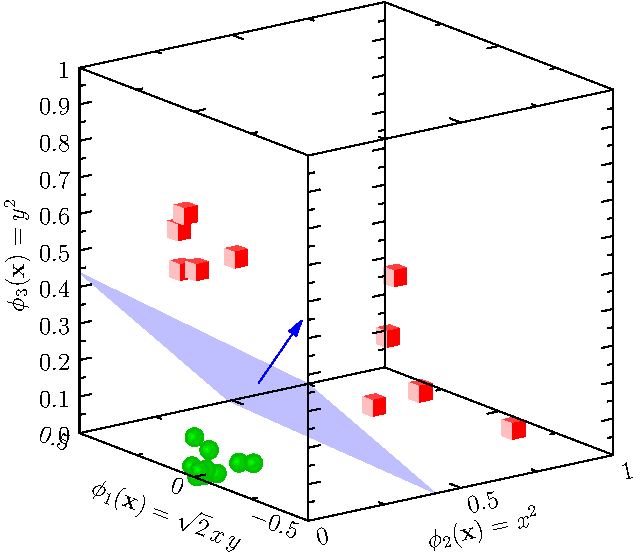
\includegraphics[height=12cm]{svm-data1}\
\end{center}

\keywords{The Kernel Trick, SVMs, Regression}


%%%%%%%%%%%%%%%%%%%%%%% Next Slide %%%%%%%%%%%%%%%%%%%%%%%
\renewcommand{\Outline}{%
\begin{slide}
\section[-1]{Outline}

\begin{minipage}{10cm}\raggedright
  \begin{enumerate}
    \outlineitem{Recap: the Kernel Trick}{kernels}
    \outlineitem{Mercer's Theorem}{eigen}
    \outlineitem{Constructing Kernels}{psdk}
    \outlineitem{Kernels for Structured Data}{structured}
    \outlineitem{Beyond Classification}{beyond}
  \end{enumerate}
\end{minipage}\hfill
\begin{minipage}{13cm}
  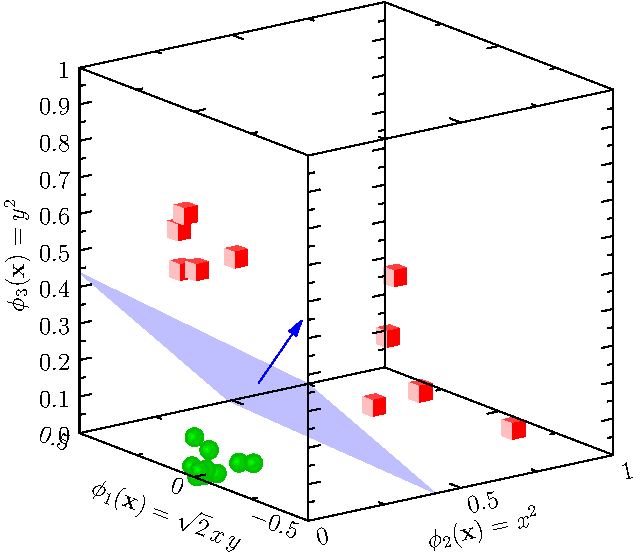
\includegraphics[width=13cm]{svm-data1}
\end{minipage}
\end{slide}
\addtocounter{outlineitem}{1}
}

\setcounter{outlineitem}{1}

%%%%%%%%%%%%%%%%%%%%%%% Next Slide %%%%%%%%%%%%%%%%%%%%%%%
\Outline % Recap
%%%%%%%%%%%%%%%%%%%%%%% Next Slide %%%%%%%%%%%%%%%%%%%%%%%

\begin{slide}
\section[-2]{Recap: the Kernel Trick}

\begin{PauseHighLight}
  \begin{itemize}\squeeze
  \item SVM kernels are functions of two variables that factorise
    \begin{align*}
      K(\bm{x},\bm{y}) = \inner{\bm{\phi}(\bm{x})}{\bm{\phi}(\bm{y})} =
      \sum_{i} \phi_i(\bm{x})\,\phi_i(\bm{y})
    \end{align*}
    with real-valued $\phi_i(\bm{x})$\pause
  \item Such a $K$ is positive semi-definite\pause{} and, conversely,
    any positive semi-definite $K$ factorises (this lecture)\pause
  \item The SVM dual problem only needs the inner products
    \begin{align*}
      \max_{\bm{\alpha}} \sum_{k=1}^m \alpha_k - \frac{1}{2}
      \sum_{k,l=1}^m \alpha_k\,\alpha_l\, y_k\,y_l\,K(\bm{x}_k,\bm{x}_l)
    \end{align*}
    subject to $\sum_{k=1}^m y_k\,\alpha_k=0$ and $0\leq \alpha_k \leq C$\pause
  \item This is the \emph{kernel trick}: we never compute
    $\bm{\phi}(\bm{x})$\pause
  \end{itemize}
\end{PauseHighLight}

\end{slide}
%%%%%%%%%%%%%%%%%%%%%%% Next Slide %%%%%%%%%%%%%%%%%%%%%%%


%%%%%%%%%%%%%%%%%%%%%%% Next Slide %%%%%%%%%%%%%%%%%%%%%%%
\Outline % Mercer's theorem
%%%%%%%%%%%%%%%%%%%%%%% Next Slide %%%%%%%%%%%%%%%%%%%%%%%

\begin{slide}
\section[-1]{Recap on Eigen Systems}

\begin{PauseHighLight}
  \begin{itemize}\squeeze
  \item Recall for a symmetric ($n\times n$) matrix $\mat{M}$ an
    eigenvector, $\bm{v}$
    \begin{align*}
      \mat{M} \, \bm{v} = \lambda \bm{v}\pause
    \end{align*}
  \item There are $n$ independent eigenvectors $\bm{v}^{(i)}$ with
    real eigenvalues $\lambda^{(i)}$\pause
  \item The eigenvectors can be chosen orthonormal:
    $\bm{v}^{(i)\tr}\bm{v}^{(j)}=0$ if $i\neq j$ ($=1$ if $i=j$)\pause
  \item Forming a matrix of eigenvectors
    $\mat{V}=(\bm{v}^{(1)},\,\bm{v}^{(2)},\, \ldots\,\bm{v}^{(n)})$ the matrix
    satisfies
    \begin{align*}
      \mat{V}^\tr \mat{V} = \mat{V}\,\mat{V}^\tr = \mat{I}\pause
    \end{align*}
  \item Such matrices are said to be orthogonal\pause
      \end{itemize}
\end{PauseHighLight}

\end{slide}
%%%%%%%%%%%%%%%%%%%%%%% Next Slide %%%%%%%%%%%%%%%%%%%%%%%

\begin{slide}
\section[-2]{Eigen Decomposition}

\begin{PauseHighLight}\squeeze
  \begin{itemize}
  \item From the eigenvalue equation $\mat{M} \, \bm{v}^{(k)} = \lambda^{(k)}
    \bm{v}^{(k)}$
     \vspace*{-0.5em}
    \begin{align*}
      \mat{M} \mat{V} &= \mat{V} \, \mat{\Lambda} & \mbox{where}\quad
      \mat{\Lambda} &= {\small
      \begin{pmatrix}
        \lambda_1 & 0 & \cdots & 0 \\
        0 & \lambda_2 & \cdots & 0 \\
        \vdots & \vdots & \ddots & \vdots \\
        0 & 0 & \cdots & \lambda_n
      \end{pmatrix}}\pause
    \end{align*}                         \vspace*{-2em}
  \item Multiplying on the right by $\mat{V}^\tr$ we get
    \begin{align*}
      \mat{M} &= \mat{V} \, \mat{\Lambda} \mat{V}^\tr = \sum_{k=1}^n
      \lambda^{(k)}\, \bm{v}^{(k)}\, \bm{v}^{(k)\tr}\pause 
    \end{align*}
    Or \vspace*{-1em}
    \begin{align*}
      M_{ij} = \sum_{k=1}^n \lambda^{(k)}\, v^{(k)}_i\, v^{(k)}_j
      \pause = \sum_{k=1}^n u^{(k)}_i\, u^{(k)}_j = \langle \bm{u}_i, \bm{u}_j \rangle
    \end{align*}
    $u^{(k)}_i = \sqrt{\lambda^{(k)}}\,v^{(k)}_i$ (real only if
    $\lambda^{(k)}\geq0$)\pauseb
  \end{itemize}
\end{PauseHighLight}

\end{slide}
%%%%%%%%%%%%%%%%%%%%%%% Next Slide %%%%%%%%%%%%%%%%%%%%%%%

\begin{slide}
\section[-2]{Limit Process}

\pb\pause
\begin{itemize}
\item Consider sampling a function at a set of
  points\pauseh\pauselevel{=1}
  \begin{center}
    \multipdf[width=0.8\linewidth]{sampleFunction}\pause
  \end{center}
\item In the limit where the number of sample points goes to infinity
  the vector more closely approximates a function\pauseh
\item The $k^{th}$ component of the vector corresponds to $f(x_k)$\pauseh
\end{itemize}

\end{slide}
%%%%%%%%%%%%%%%%%%%%%%% Next Slide %%%%%%%%%%%%%%%%%%%%%%%

\begin{slide}
\section[-2]{Linear Operators}

\begin{PauseHighLight}
  \begin{itemize}\squeeze
  \item Recall a linear operator on functions, $\mathcal{T}[f(x)]$,
    can often be represented by a kernel
    \begin{align*}
      \mathcal{T}[f(x)] = \int_{y\in\mathcal{I}} K(x,y)\,f(y)\,\dd
      y\pause \approx \Delta \sum_{j=1}^n K(x, y_j)\, f(y_j)\pauseb
    \end{align*}
    \begin{center}
      \multipdf[width=0.7\linewidth]{approxKernel}\pauseb
    \end{center}
  This is just a matrix equation with $M_{ij}=\Delta\,K(x_i, y_j)$\pause
  \end{itemize}
\end{PauseHighLight}

\end{slide}
%%%%%%%%%%%%%%%%%%%%%%% Next Slide %%%%%%%%%%%%%%%%%%%%%%%

\begin{slide}
\section{Eigenfunctions}

\begin{PauseHighLight}
  \begin{itemize}
  \item By analogy for a symmetric function of two variables we can
    define an \textit{eigenfunction}
    \begin{align*}
      \int K(\bm{x}, \bm{y})\, \psi(\bm{y}) \, \dd \, \bm{y} = \lambda
      \, \psi(\bm{x})\pause
    \end{align*}
  \item In general there will be a denumerable set of eigenfunctions
    $\psi^{(k)}(\bm{x})$ where
    \begin{align*}
      K(\bm{x}, \bm{y}) = \sum_k \lambda^{(k)}\,
      \psi^{(k)}(\bm{x})\,\psi^{(k)}(\bm{y})\pause
    \end{align*}
  \item For a positive semi-definite kernel (on a bounded domain) this
    is \emph{Mercer's theorem}\pause
  \end{itemize}
\end{PauseHighLight}

\end{slide}
%%%%%%%%%%%%%%%%%%%%%%% Next Slide %%%%%%%%%%%%%%%%%%%%%%%

\begin{slide}
\section[-2]{From Eigenfunctions to Features}

\begin{PauseHighLight}
  \begin{itemize}
  \item If we define $\phi^{(k)}(\bm{x}) = \sqrt{\lambda^{(k)}} \psi^{(k)}(\bm{x})$
    then
    \begin{align*}
      K(\bm{x}, \bm{y}) &= \sum_k \lambda^{(k)}\,
      \psi^{(k)}(\bm{x})\,\psi^{(k)}(\bm{y})
      = \sum_k \phi^{(k)}(\bm{x})\,\phi^{(k)}(\bm{y})\pause
    \end{align*}
  \item This is the definition of an SVM kernel we started with\pause
  \item Note that for $\phi^{(k)}(\bm{x})$ to be real $\lambda^{(k)}\geq 0$ for
    all $k$\pause
  \item If $\lambda^{(k)} < 0$ then $\langle \bm{\phi}(\bm{x}),
    \bm{\phi}(\bm{x}) \rangle = \len{\phi(\bm{x})}^2$ might be
    negative and  ``distance'' between points in the
    extended feature space can be negative!\pause
  \item If we use a kernel that isn't positive semi-definite then the
    Hessian of the dual objective need not be negative
    semi-definite: the objective can be unbounded, with $\bm{\alpha}$
    diverging\pause
  \end{itemize}
\end{PauseHighLight}

\end{slide}

%%%%%%%%%%%%%%%%%%%%%%% Next Slide %%%%%%%%%%%%%%%%%%%%%%%
\Outline % Constructing kernels
%%%%%%%%%%%%%%%%%%%%%%% Next Slide %%%%%%%%%%%%%%%%%%%%%%%

\begin{slide}
\section{Positive Semi-Definite Kernels}

\begin{PauseHighLight}
  \begin{itemize}
  \item Kernels (or matrices) that have eigenvalues $\lambda^{(k)}\geq0$ are
    called positive semi-definite\pause
  \item (If the eigenvalues are strictly positive $\lambda^{(k)}>0$ the
    kernels or matrices are called positive definite)\pause
  \item Positive semi-definite kernels can always be decomposed into a
    sum of real functions
    \begin{align*}
      K(\bm{x}, \bm{y}) &= \inner{\bm{\phi}(\bm{x})}{\bm{\phi}(\bm{y})}\pause
    \end{align*}
  \end{itemize}
\end{PauseHighLight}


\end{slide}
%%%%%%%%%%%%%%%%%%%%%%% Next Slide %%%%%%%%%%%%%%%%%%%%%%%

\begin{slide}
\section[-1]{Properties of Positive Semi-Definiteness}

\begin{PauseHighLight}
  \begin{itemize}
  \item Since 
    \begin{align*}
      K(\bm{x}, \bm{y}) =  \inner{\strut\bm{\phi}(\bm{x})}{\bm{\phi}(\bm{y})}\pause
    \end{align*}
  \item An immediate consequence is that for any function $f(\bm{x})$
   \begin{align*}
      \hspace*{-2em}\int f(\bm{x})\, K(\bm{x}, \bm{y})\, f(\bm{y})\,\dd\bm{x}\, \dd
       \bm{y} &= \int f(\bm{x}) \,
                \inner{\strut\bm{\phi}(\bm{x})}{\bm{\phi}(\bm{y})}
                \, f(\bm{y})\,\dd\bm{x}\, \dd \bm{y}\pause  \\
      &=\inner{\int f(\bm{x})\,
        \bm{\phi}(\bm{x})\,\dd\bm{x}}{\int f(\bm{y})\,
        \bm{\phi}(\bm{y})\,\dd\bm{y}}\pauseb \\
     &= \left\| \int f(\bm{x})\,
        \bm{\phi}(\bm{x})\,\dd\bm{x}\right\|^2 \pauseb \geq 0\pauseb
    \end{align*}
  \end{itemize}
\end{PauseHighLight}


\end{slide}
%%%%%%%%%%%%%%%%%%%%%%% Next Slide %%%%%%%%%%%%%%%%%%%%%%%

\begin{slide}
\section[-2]{Positive Semi-Definiteness}

\begin{PauseHighLight}
  \begin{itemize}\squeeze
  \item The following statements are equivalent
    \begin{itemize}
    \item $K(\bm{x}, \bm{y})$ is positive semi-definite (written
      $K(\bm{x}, \bm{y})\succeq 0$)\pause
    \item The eigenvalues of $K(\bm{x}, \bm{y})$ are non-negative\pause
    \item The kernel can be written
      \begin{align*}
        K(\bm{x}, \bm{y}) =  \inner{\strut\bm{\phi}(\bm{x})}{\bm{\phi}(\bm{y})}
      \end{align*}
      where the $\phi^{(k)}(\bm{x})$'s are real functions\pause
    \item For any real function $f(\bm{x})$
      \begin{align*}
        \int f(\bm{x})\, K(\bm{x}, \bm{y}) \, f(\bm{y})
         \, \dd \bm{x}  \, \dd \bm{y} \geq 0\pause
      \end{align*}
    \item For any points $\bm{x}_1,\ldots,\bm{x}_n$ the \emph{Gram
        matrix} with elements $K_{ij}=K(\bm{x}_i,\bm{x}_j)$ is positive
      semi-definite\pause
    \end{itemize}
  \end{itemize}
\end{PauseHighLight}

\end{slide}
%%%%%%%%%%%%%%%%%%%%%%% Next Slide %%%%%%%%%%%%%%%%%%%%%%%

\begin{slide}
\section[-1]{Adding Kernels}

\begin{PauseHighLight}
  \begin{itemize}
  \item We can construct SVM kernels from other kernels\pause
  \item If $K_1(\bm{x}, \bm{y})$ and  $K_2(\bm{x}, \bm{y})$ are valid
    kernels then so is $K_3(\bm{x}, \bm{y}) = K_1(\bm{x}, \bm{y}) +
    K_2(\bm{x}, \bm{y})$
    \begin{align*}
      \hspace*{-1em}Q &= \int f(\bm{x})\, K_3(\bm{x}, \bm{y}) \, f(\bm{y})
      \, \dd \bm{x}  \, \dd \bm{y} \\
      &=\int f(\bm{x})\, \left( \strut K_1(\bm{x}, \bm{y}) + K_2(\bm{x},
      \bm{y}) \right)  f(\bm{y}) \, \dd \bm{x}  \, \dd \bm{y} \\
      &=\int f(\bm{x})\, K_1(\bm{x}, \bm{y}) \, f(\bm{y})
      \, \dd \bm{x}  \, \dd \bm{y} +
      \int f(\bm{x})\, K_2(\bm{x}, \bm{y}) \, f(\bm{y})
      \, \dd \bm{x}  \, \dd \bm{y}
      \geq 0   \pause
    \end{align*}
  \item If $K(\bm{x}, \bm{y})$ is a valid kernel so is $c\,K(\bm{x},
    \bm{y})$ for $c>0$\pause
  \end{itemize}
\end{PauseHighLight}

\end{slide}
%%%%%%%%%%%%%%%%%%%%%%% Next Slide %%%%%%%%%%%%%%%%%%%%%%%

\begin{slide}
\section[-2]{Product of Kernels}

\begin{PauseHighLight}
  \begin{itemize}
  \item If $K_1(\bm{x}, \bm{y})$ and  $K_2(\bm{x}, \bm{y})$ are valid
    kernels then so is $K_3(\bm{x}, \bm{y}) = K_1(\bm{x}, \bm{y})\,
    K_2(\bm{x}, \bm{y})$\pause
  \item Writing {\small
    \begin{align*}
      K_1(\bm{x}, \bm{y}) &= \sum_i \phi^{(1)}_i(\bm{x})\,
    \phi^{(1)}_i(\bm{y}), &
                           K_2(\bm{x}, \bm{y}) &= \sum_j \phi^{(2)}_j(\bm{x})\,
    \phi^{(2)}_j(\bm{y})
    \end{align*}}
    then
    \begin{align*}
      K_3(\bm{x}, \bm{y})
      &= \sum_{i,j} \phi^{(1)}_i(\bm{x})\,\phi^{(1)}_i(\bm{y})\,
      \phi^{(2)}_j(\bm{x})\,\phi^{(2)}_j(\bm{y}) \pause\\
      &= \sum_{i,j} \phi^{(3)}_{ij}(\bm{x})\,
      \phi^{(3)}_{ij}(\bm{y})\pauseb = \inner{\bm{\phi}^{(3)}(\bm{x})}{\bm{\phi}^{(3)}(\bm{y})}\pauseb
    \end{align*}\pauselevel{=3}
    where $\phi^{(3)}_{ij}(\bm{x}) = \phi^{(1)}_i(\bm{x})\,\phi^{(2)}_j(\bm{x})$\pauseb
  \end{itemize}
\end{PauseHighLight}

\end{slide}
%%%%%%%%%%%%%%%%%%%%%%% Next Slide %%%%%%%%%%%%%%%%%%%%%%%

\begin{slide}
\section{Exponentiating Kernels}

\begin{PauseHighLight}
  \begin{itemize}
  \item If $K(\bm{x}, \bm{y})$ is a valid kernel so is 
    $K^n(\bm{x}, \bm{y})$ (by induction)\pause
    \begin{itemize}\squeeze
    \item Assume $K(\bm{x}, \bm{y}) \succeq 0$ this satisfies base case\pause
    \item If $K^{n-1} (\bm{x}, \bm{y})\succeq 0$ then
      \begin{align*}
        K^{n}(\bm{x}, \bm{y}) = K^{n-1} (\bm{x}, \bm{y}) \, K(\bm{x}, \bm{y})\succeq 0\pause
      \end{align*}
    \end{itemize}
  \item and $\exp(K(\bm{x}, \bm{y}))$ is also a valid kernel since
    \begin{align*}
      \e{K(\bm{x}, \bm{y})} = \sum_{i=0}^\infty \frac{1}{i!} K^i(\bm{x}, \bm{y})
      = 1 + K(\bm{x}, \bm{y}) + \frac{1}{2} K^2(\bm{x}, \bm{y}) + \cdots
    \end{align*}
    but each term in the sum is a kernel (the constant $1$ has
    $\phi(\bm{x})=1$)\pause
  \end{itemize}
\end{PauseHighLight}

\end{slide}
%%%%%%%%%%%%%%%%%%%%%%% Next Slide %%%%%%%%%%%%%%%%%%%%%%%

\begin{slide}
\section[-2]{Polynomial Kernels}

\begin{PauseHighLight}
  \begin{itemize}
  \item A constant $c\geq0$ is a kernel: $c = \sqrt{c}\,\sqrt{c}$, so
    $\phi(\bm{x})=\sqrt{c}$\pause
  \item $\bm{x}^\tr\bm{y}$ is a kernel (with $\bm{\phi}(\bm{x})=\bm{x}$),
    so the sum $c+\bm{x}^\tr\bm{y}$ is too\pause
  \item Hence the \emph{polynomial kernel}
    \begin{align*}
      K(\bm{x},\bm{y}) = \left(c+\bm{x}^\tr\bm{y}\right)^d
    \end{align*}
    is a kernel for $d=1,\,2,\,\ldots$\pause
  \item Its features $\bm{\phi}(\bm{x})$ are all the monomials of the
    $x_i$ of degree up to $d$ (suitably weighted)\pause
  \item $c=0$, $d=2$ is the quadratic kernel from the last
    lecture\pause
  \end{itemize}
\end{PauseHighLight}

\end{slide}
%%%%%%%%%%%%%%%%%%%%%%% Next Slide %%%%%%%%%%%%%%%%%%%%%%%

\begin{slide}
\section[-2]{RBF Kernel}

\begin{PauseHighLight}
  \begin{itemize}
  \item Now $\bm{x}^\tr\bm{y} = \inner{\bm{x}}{\bm{y}}$ is a valid
    kernel because it is an inner product of functions $\bm{\phi}(\bm{x}) =
    \bm{x}$\pause
  \item For $\gamma>0$ we have $2\,\gamma\,\bm{x}^\tr\bm{y}\succeq 0$\pause
  \item Thus $\exp(2\,\gamma\,\bm{x}^\tr\bm{y}) \succeq 0$\pause
  \item If $K(\bm{x},\bm{y})\succeq0$ then
    $g(\bm{x})\,K(\bm{x},\bm{y})\,g(\bm{y}) \succeq 0$\pause
    {\small
    \begin{align*}
      \int f(\bm{x})\, g(\bm{x})\,K(\bm{x}, \bm{y}) \,g(\bm{y})\,
      f(\bm{y}) \, \dd \bm{x} \dd \bm{y}  \pause= \int
      h(\bm{x})\,K(\bm{x}, \bm{y}) \,h(\bm{y})\, \dd \bm{x} \dd
      \bm{y}\pauseb \geq 0 \pauseb \pauselevel{=6}
    \end{align*}}
    where $f(\bm{x})\, g(\bm{x})= h(\bm{x})$\pauseb\pauselevel{=8}
    \begin{align*}
      \e{-\gamma\,\bm{x}^\tr\bm{x}}\,\e{2\,\gamma\,\bm{x}^\tr\bm{y}}
      \,\e{- \gamma\,\bm{y}^\tr\bm{y}}\pauseb
      &= \e{-\gamma\,\|\bm{x}-\bm{y}\|^2}\pauseb \succeq
        0\pauseb
    \end{align*}
  \end{itemize}
\end{PauseHighLight}

\end{slide}

%%%%%%%%%%%%%%%%%%%%%%% Next Slide %%%%%%%%%%%%%%%%%%%%%%%
\Outline % Structured data
%%%%%%%%%%%%%%%%%%%%%%% Next Slide %%%%%%%%%%%%%%%%%%%%%%%

\begin{slide}
\section{Other Kernels}

\begin{PauseHighLight}
  \begin{itemize}
  \item The success of SVMs has meant that researchers try to increase
    the area of application\pause
  \item The condition that an SVM kernel must be positive semi-definite
    is quite restrictive\pause
  \item The key to finding new kernels is to use the properties of
    kernels to build more complicated kernels from simpler ones\pause
  \item There has been a cottage industry of researchers finding smart
    kernels for complicated data\pause
  \item One area where SVMs were very important is document
    classification, which requires comparing strings\pause
  \end{itemize}
\end{PauseHighLight}

\end{slide}
%%%%%%%%%%%%%%%%%%%%%%% Next Slide %%%%%%%%%%%%%%%%%%%%%%%

\begin{slide}
\section[-1]{Spectrum Kernel}

\begin{PauseHighLight}
  \begin{itemize}
  \item A simple way to compare documents is to collect a histogram of
    all occurrences of substrings of length $\ell$\pause
  \item This is known as an $\ell$-spectrum\pause
  \item The $\ell$-spectrum kernel is the inner product of the two
    histograms
    {\small
    \begin{align*}
      s &= \mbox{\tt statistics} & \mathcal{S}_3(s) &= \{\mathtt{sta, tat, ati, tis,
      ist, sti, tic, ics}\}
      \\
      t &= \mbox{\tt computation} & \mathcal{S}_3(t) &= \{\mathtt{com, omp,
      mpu, put, uta, tat, ati, tio, ion}\}\pause
    \end{align*}}
  \item $K(s,t) = 1\times1+1\times1 = 2$ (``\texttt{tat}'' and
    ``\texttt{ati}'' each occur once in both)\pause
  \end{itemize}
\end{PauseHighLight}

\end{slide}
%%%%%%%%%%%%%%%%%%%%%%% Next Slide %%%%%%%%%%%%%%%%%%%%%%%

\begin{slide}
\section{All Subsequences Kernel}

\begin{PauseHighLight}
  \begin{itemize}
  \item A more sophisticated kernel counts all of the common
    subsequences (not necessarily contiguous) of two documents\pause
  \item Naively this would take an exponential amount of time to
    compute\pause
  \item Using clever dynamic-programming techniques this can be done
    relatively efficiently\pause
  \item Gap-weighted versions down-weight subsequences that are spread
    out over long gaps\pause
  \end{itemize}
\end{PauseHighLight}

\end{slide}
%%%%%%%%%%%%%%%%%%%%%%% Next Slide %%%%%%%%%%%%%%%%%%%%%%%

\begin{slide}
\section{Other Kernel Applications}

\begin{PauseHighLight}
  \begin{itemize}
  \item String kernels for comparing subsequences are used in
    bioinformatics\pause
  \item Kernels have been developed for comparing trees (e.g. for
    computer program evaluation, XML, etc.)\pause
  \item Kernels have also been developed for comparing graphs (e.g. for
    comparing chemicals based on their molecular graph)\pause
  \end{itemize}
\end{PauseHighLight}

\end{slide}
%%%%%%%%%%%%%%%%%%%%%%% Next Slide %%%%%%%%%%%%%%%%%%%%%%%

\begin{slide}
\section{Fisher Kernels}

\begin{PauseHighLight}
  \begin{itemize}
  \item In an attempt to build kernels that capture more domain
    knowledge, kernels are constructed from other learning
    machines\pause
  \item An example is the \emph{Fisher kernel}, whose features are the
    gradients of the log-likelihood of a generative model (e.g. a
    Hidden Markov Model, HMM) trained on the data\pause
  \item These tend to have better discriminative power than the
    underlying model (HMM), and a better feature set than an SVM
    using a generic kernel\pause
  \end{itemize}
\end{PauseHighLight}

\end{slide}

%%%%%%%%%%%%%%%%%%%%%%% Next Slide %%%%%%%%%%%%%%%%%%%%%%%
\Outline % Beyond
%%%%%%%%%%%%%%%%%%%%%%% Next Slide %%%%%%%%%%%%%%%%%%%%%%%

\begin{slide}
\section[-2]{Regression with Margins}

\begin{PauseHighLight}
  \begin{itemize}
  \item SVMs can be modified to perform regression
    \begin{center}
      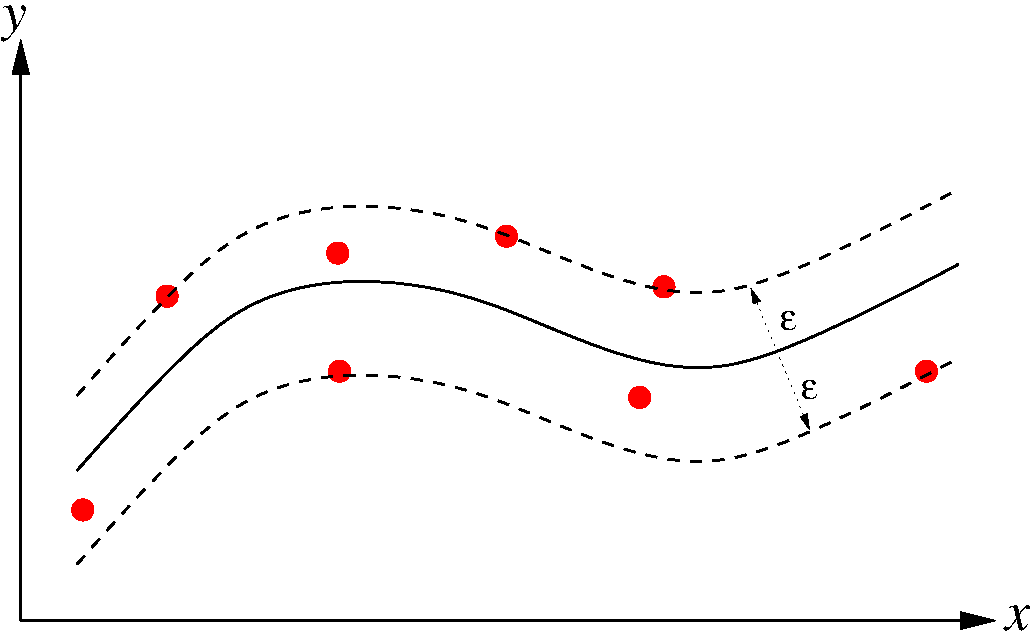
\includegraphics[width=0.9\linewidth]{svm-regress}
    \end{center}
  \end{itemize}
\end{PauseHighLight}

\end{slide}
%%%%%%%%%%%%%%%%%%%%%%% Next Slide %%%%%%%%%%%%%%%%%%%%%%%

\begin{slide}
\section{Error Functions}

\begin{PauseHighLight}
  \begin{itemize}
  \item Can introduce slack variables with different errors
    \begin{center}
      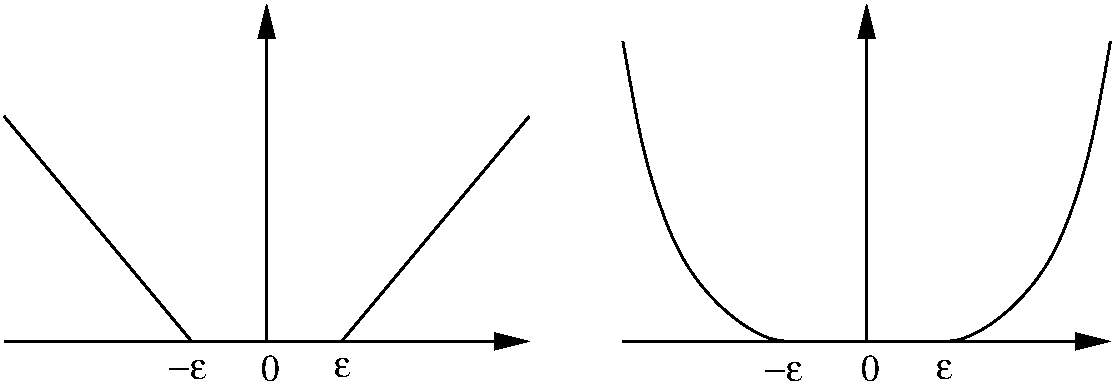
\includegraphics[width=0.9\linewidth]{svm-regression}
    \end{center}
  \item This can be transformed to a quadratic programming problem
  \end{itemize}
\end{PauseHighLight}

\end{slide}
%%%%%%%%%%%%%%%%%%%%%%% Next Slide %%%%%%%%%%%%%%%%%%%%%%%

\begin{slide}
\section{Ridge Regression Using Kernels}

\begin{PauseHighLight}
  \begin{itemize}
  \item We can also solve regression problems without using margins\pause
  \item Kernel ridge regression minimises
    \begin{align*}
      \min_{\bm{w}} \; \eta\,\| \bm{w} \|^2 + \sum_{i=1}^m \left( y_i -
      \bm{w}^\tr \bm{\phi}(\bm{x}_i) \right)^2\pause
    \end{align*}
    where $\eta\,\| \bm{w} \|^2$ is a regularisation term\pause
  \item The optimal $\bm{w}$ lies in the span of the
    $\bm{\phi}(\bm{x}_i)$ (any other component only increases
    $\|\bm{w}\|^2$), so $\bm{w} = \sum_i \alpha_i \,\bm{\phi}(\bm{x}_i)$\pause
  \item This gives $\bm{\alpha} = (\mat{K}+\eta\,\mat{I})^{-1}\bm{y}$,
    with $\mat{K}$ the Gram matrix, and predictions
    $f(\bm{x}) = \sum_i \alpha_i\, K(\bm{x}_i,\bm{x})$\pause
  \end{itemize}
\end{PauseHighLight}

\end{slide}
%%%%%%%%%%%%%%%%%%%%%%% Next Slide %%%%%%%%%%%%%%%%%%%%%%%

\begin{slide}
\section{Kernel Methods}

\begin{PauseHighLight}
  \begin{itemize}
  \item Kernel methods where we project into an extended feature space
    are used with other linear algorithms
    \begin{itemize}
    \item Kernel Fisher discriminant analysis (KFDA)
    \item Kernel principal component analysis (KPCA)
    \item Kernel canonical correlation analysis (KCCA)
    \item Gaussian Processes\pause
    \end{itemize}
  \item These are also extremely powerful machine learning algorithms\pause
  \end{itemize}
\end{PauseHighLight}

\end{slide}
%%%%%%%%%%%%%%%%%%%%%%% Next Slide %%%%%%%%%%%%%%%%%%%%%%%

\begin{slide}
\section[-1]{Summary}

\begin{PauseHighLight}
  \begin{itemize}
  \item SVMs require a positive semi-definite kernel function\pause
  \item These can be built from simpler functions\pause
  \item There was a cottage industry of people creating new kernels
    for different applications\pause
  \item SVMs are just one example of a host of machines that
    \begin{itemize}
    \item use the kernel trick
    \item often use linear constraints
    \item tend to be convex optimisation problems\pause
    \end{itemize}
  \end{itemize}
\end{PauseHighLight}

\end{slide}

%%% Local Variables:
%%% TeX-master: "lectures"
%%% End:

\end{document}
